% This is a draft of the coming paper "Multiple Round Ballot Polling Risk-Limiting Audit Simulations".
% 2021.
%
\documentclass{beamer}
%
\usepackage{float}
\usepackage{xspace}
\usepackage{graphicx}
\graphicspath{{./imgs/}}
\usepackage{comment}
\usepackage{listings,hyperref}
\usepackage{cite}

% \usepackage{graphicx}  --> Used for displaying a sample figure. If possible, figure files should
% be included in EPS format.
%
% If you use the hyperref package, please uncomment the following line
% to display URLs in blue roman font according to Springer's eBook style:
% \renewcommand\UrlFont{\color{blue}\rmfamily}


% nice looking audit titles
\newcommand{\Minerva}{\textsc{Minerva}\xspace}
\newcommand{\B}{{{B2}}\xspace}
\newcommand{\R}{{{R2}}\xspace}
\newcommand{\BRAVO}{\textsc{Bravo}\xspace}

\usepackage{color}
\definecolor{green}{rgb}{0.31, 0.78, 0.47}
\newcommand{\fpo}[1]{\textcolor{green}{#1}}

\def\code#1{\texttt{#1}}

\begin{document}
\lstset{language=Python}
%
\title{Simulations of Ballot Polling Risk-Limiting Audits}
%add \thanks{} within the title brackets if want to refer to supporting organization ^^
%
%\titlerunning{Abbreviated paper title}
% If the paper title is too long for the running head, you can set
% an abbreviated paper title here
%
\author{Oliver Broadrick\inst{1} \and
Sarah Morin\inst{1} \and
Grant McClearn\inst{2}\\ \and Neal McBurnett \and Poorvi L. Vora\inst{1} \and
Filip Zag{\'o}rski\inst{3}\inst{4}}
%
% First names are abbreviated in the running head.
% If there are more than two authors, 'et al.' is used.
%
\institute{\inst{1} Department of Computer Science, The George Washington University (odbroadrick@gmail.com)
%\thanks{Supported in part by NSF Award 2015253} 
\and \inst{2} Department of Computer Science, Stanford University (grantmcc@stanford.edu)
\and \inst{3} Wroclaw University of Science and Technology (filip.zagorski@gmail.com)
%\thanks{Author was partially supported by Polish National Science Centre contract number DEC-2013/09/D/ST6/03927} and 
\and \inst{4} Votifica
}
%

%\maketitle              % typeset the header of the contribution
\frame{\titlepage}
%

\begin{frame}
\frametitle{Outline}

\begin{itemize}
\item Risk-Limiting Audits
\begin{itemize}
\item \BRAVO and \Minerva
\end{itemize}
\item Experiments
\item Results
\begin{itemize}
\item Stopping Probability
\item Risk
\item Number of Ballots
\end{itemize}
\item Discussion and Future Work
\end{itemize}

\end{frame}


\begin{frame}
\frametitle{Post-tabulation audits}

\begin{itemize}
\item Scanning machines are used to tabulate ballots
\begin{itemize}
\item Cannot trust the machines: bugs, configuration errors, hacking
\end{itemize}
\item Post-tabulation audits
\item Risk-Limiting Audits
\end{itemize}
\end{frame}

\begin{frame}
\frametitle{Risk-Limiting Audits}

\begin{itemize}
\item Risk-Limiting Audit (RLA) is a post-tabulation audit that manualy
checks a random sample of voters' ballots
\item Relies on a voter-verified paper trail
\item Sketch:
\begin{enumerate}
\item election results announced
\item sample ballots randomly
\item check if the sample is 'statistically similar' to the announced tally
\begin{itemize}
\item "Yes" - correct - stop the audit
\item "No" - incorrect - proceed to a full hand count
\item "Don't know yet" - undetermined - draw more samples (goto: 2)
\end{itemize}
\end{enumerate}
\end{itemize}
\end{frame}

\begin{frame}
\frametitle{\BRAVO}
\begin{itemize}
\item Most commonly used ballot polling RLA
\item In the two candidate case is an instance of Wald's Sequential Probability Ratio Test (SPRT)
\item Is thus the most efficient RLA when ballots are drawn sequentially (i.e. ballot-by-ballot)
\item Real audits are performed in rounds for which \BRAVO can be implemented as:
\begin{itemize}
\item Selection-Ordered (SO) \BRAVO
\item End-of-Round (EoR) \BRAVO
\end{itemize}
\end{itemize}
\end{frame}

\begin{frame}
\frametitle{\Minerva}
\begin{itemize}
\item Recent RLA designed for round-by-round use
\item Uses a ratio of the \emph{tails} of the probability distributions used in \BRAVO
\item Known to require half the number of ballots as EoR \BRAVO in a first round to achieve a large ($0.90$) probability of stopping
\item Unknown how the audits compare for smaller stopping probability or for rounds after the first
\end{itemize}
\end{frame}

\begin{frame}
\frametitle{Experiments}
\begin{itemize}
\item Use simulations to provide evidence for theoretical claims
\item R2B2 software library for round-by-round and ballot-by-ballot RLAs
\item Simulate RLAs for election results from the 2020 Presidential election (all margins above $0.05$)
\begin{itemize}
\item $10000=10^4$ trials assuming the underlying election is as announced
\item $10000=10^4$ trials assuming the underlying election is a tie
\end{itemize}
\item Risk limit: $10\%$
\item Round schedules:
\begin{itemize}
\item \BRAVO round sizes to achieve a chosen probability of stopping in each round given that the audit has already reached that round
\item \Minerva first round sizes to achieve a chosen probability of stopping, and subsequent round sizes found by multiplying the previous round size by a constant ($1.5$ and $1$)
\end{itemize}
\item Stopping probabilities: $0.90$ and $0.25$
\end{itemize}
\end{frame}

\begin{frame}
\frametitle{Experiments}
\begin{definition}
An audit $\mathcal{A}$ takes a sample of ballots $X$ as input and gives as output either
(1) $Correct$: the audit is complete, or (2) $Uncertain$: continue the audit.
\end{definition}

\begin{itemize}
\item Binary hypothesis test: $H_0$ (a tie) and $H_a$ (announced results)
\end{itemize}

\begin{definition}[Risk]
The maximum risk $R$ of audit $\mathcal{A}$ with sample $X\in \{0,1\}^*$ drawn from 
the true underlying distribution of ballots is
$R(\mathcal{A})=\Pr[\mathcal{A}(X)=Correct \mid H_0].$
\end{definition}

\begin{definition}[Risk Limiting Audit ($\alpha$-RLA)]
An audit $\mathcal{A}$ is a Risk Limiting Audit with 
risk limit $\alpha$ iff 
$R(\mathcal{A}) \le \alpha.$
\end{definition}
\end{frame}

\begin{frame}
\frametitle{Experiments}
\begin{definition}[Stopping Probability]
The stopping probability $S_j$ of an audit $\mathcal{A}$ in round $j$ is 
$S_j(\mathcal{A})=$
$$\Pr[\mathcal{A}(X)=Correct ~in~round~j~\land \mathcal{A}(X) \neq Correct ~previously \mid H_a]$$
\end{definition}

\begin{definition}[Cumulative Stopping Probability]
The cumulative stopping probability $C_j$ of an audit $\mathcal{A}$ in round $j$ is $C_j(\mathcal{A})= \sum_{i=1}^j S_j$
\end{definition}

\begin{definition}[Conditional Stopping Probability]
The conditional stopping probability  of an audit $\mathcal{A}$ in round $j$ is 
$\chi_j (\mathcal{A})=$
$$\Pr[\mathcal{A}(X)=Correct ~in~round~j~\mid H_a \land \mathcal{A}(X) \neq Correct ~previously]$$
\end{definition}
\end{frame}

\begin{frame}
\frametitle{Results: Stopping Probability ($\chi_1=0.9$)}

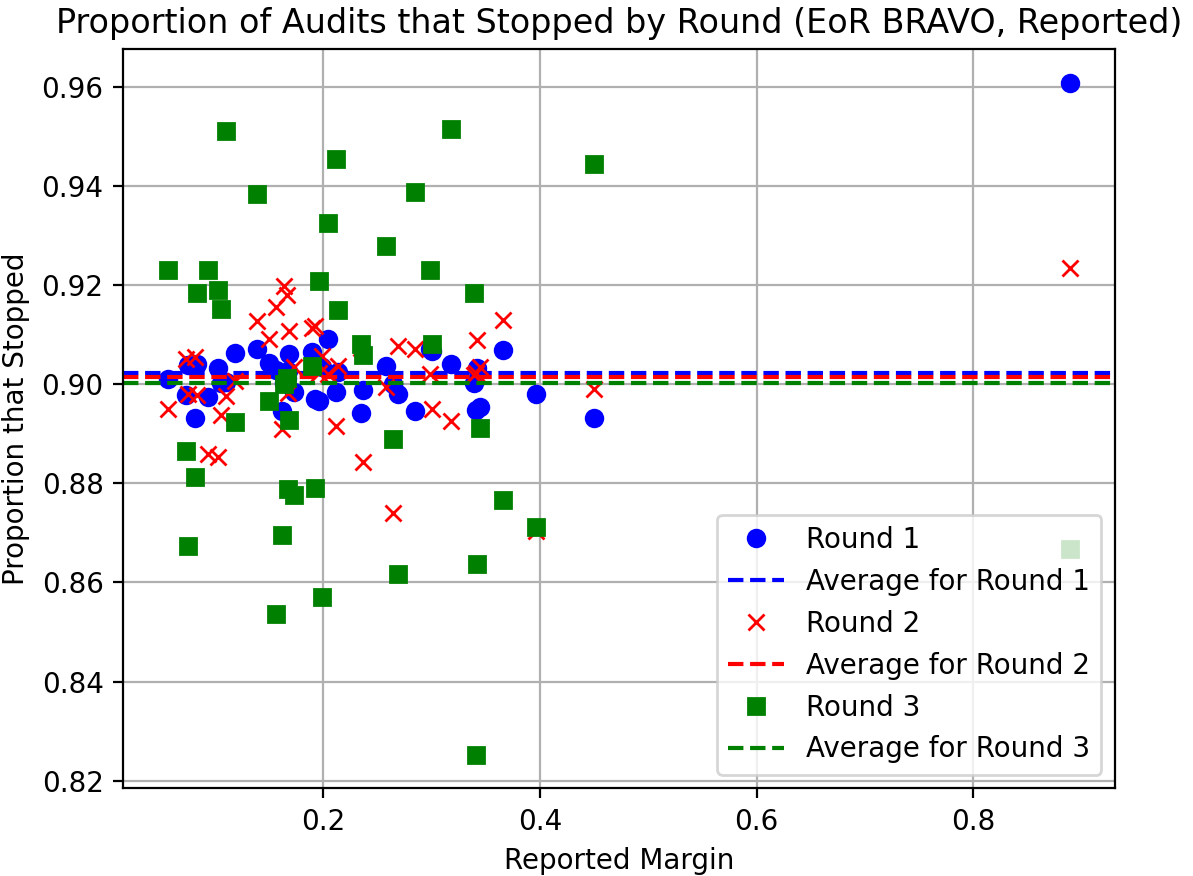
\includegraphics[width=0.5\textwidth]{eor_bravo_90perc_10^4_corrected/sprob_first_three_cropped.png}
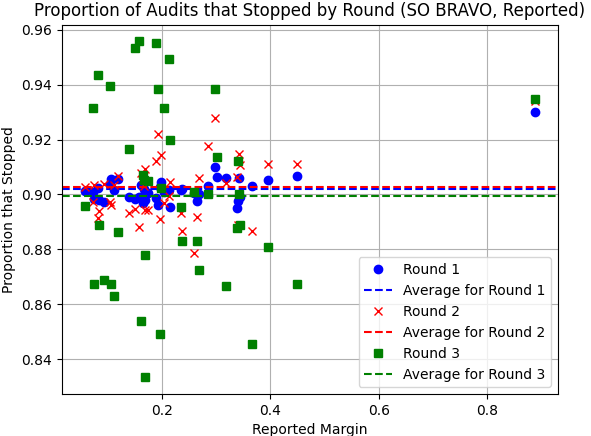
\includegraphics[width=0.5\textwidth]{so_bravo_90perc_10^4/sprob_first_three.png}

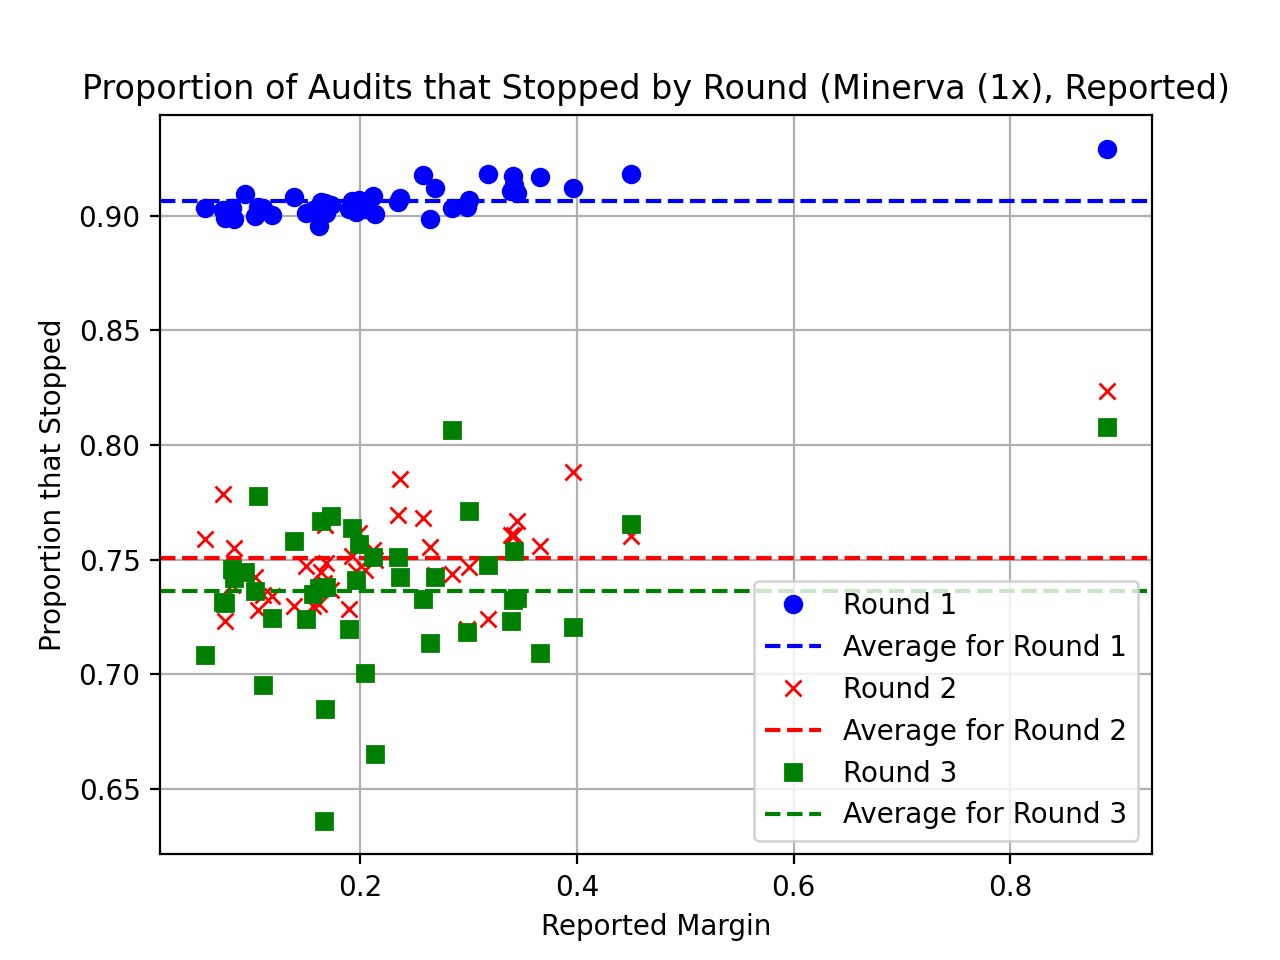
\includegraphics[width=0.5\textwidth]{minerva_multiround_1x_10^4/sprobs_first_three.png}
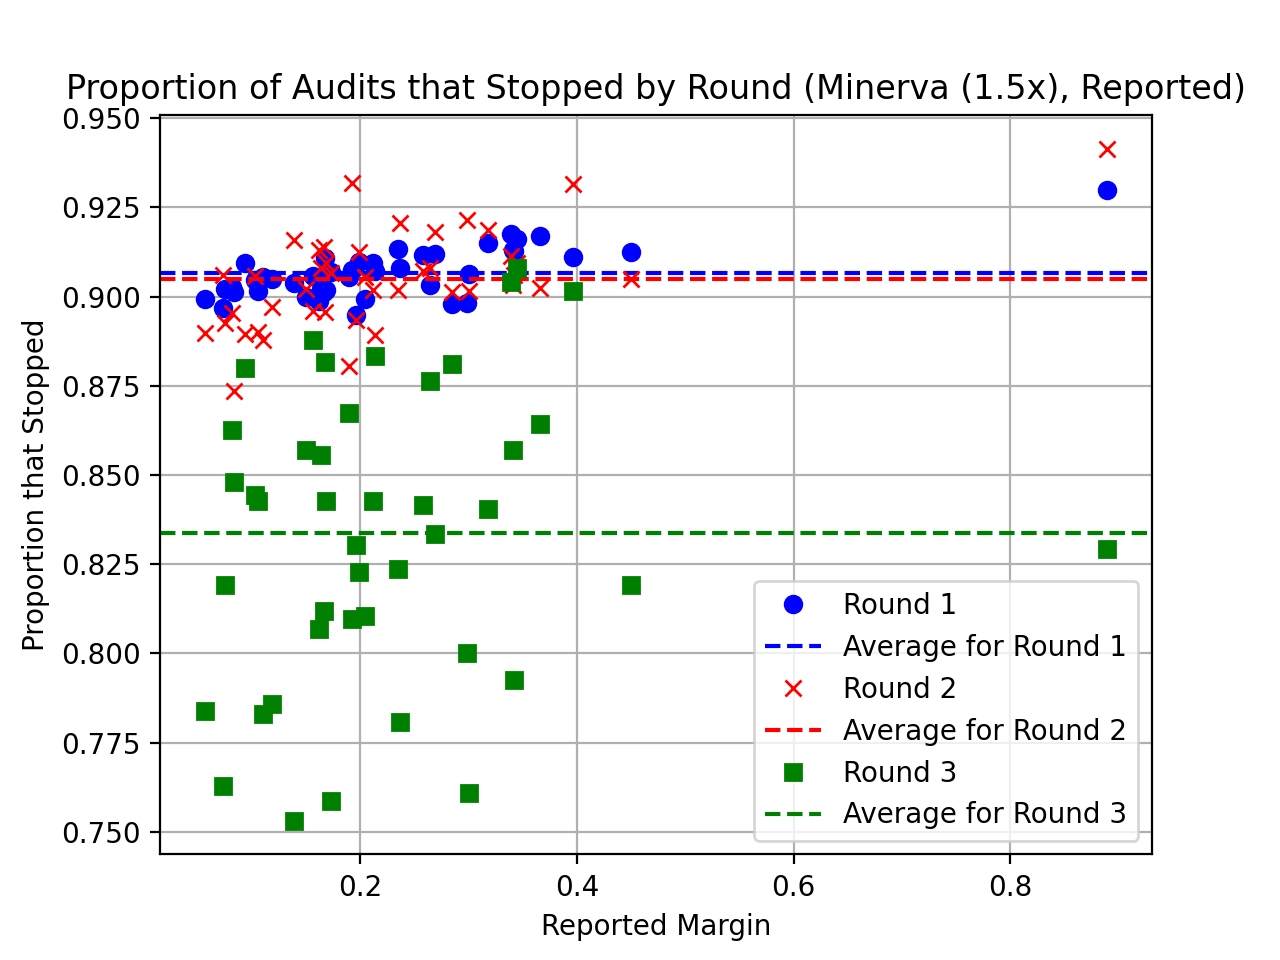
\includegraphics[width=0.5\textwidth]{minerva_multiround_1p5x_10^4/sprobs_first_three.png}
\end{frame}

\begin{frame}
\frametitle{Results: Stopping Probability ($\chi_1=0.25$)}

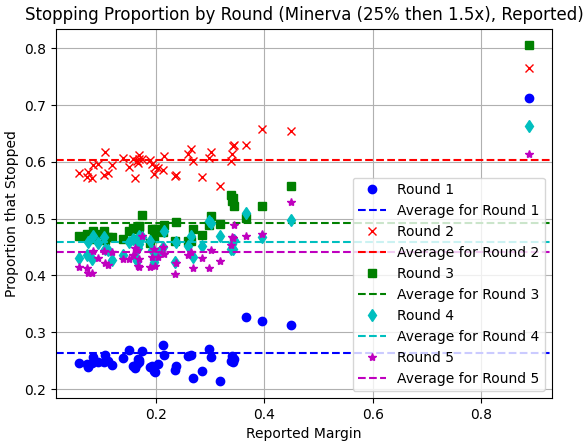
\includegraphics[width=1\textwidth]{minerva25percthen1p5_sprob.png}
\end{frame}


\begin{frame}
\frametitle{Results: Risk}

\centering
\noindent 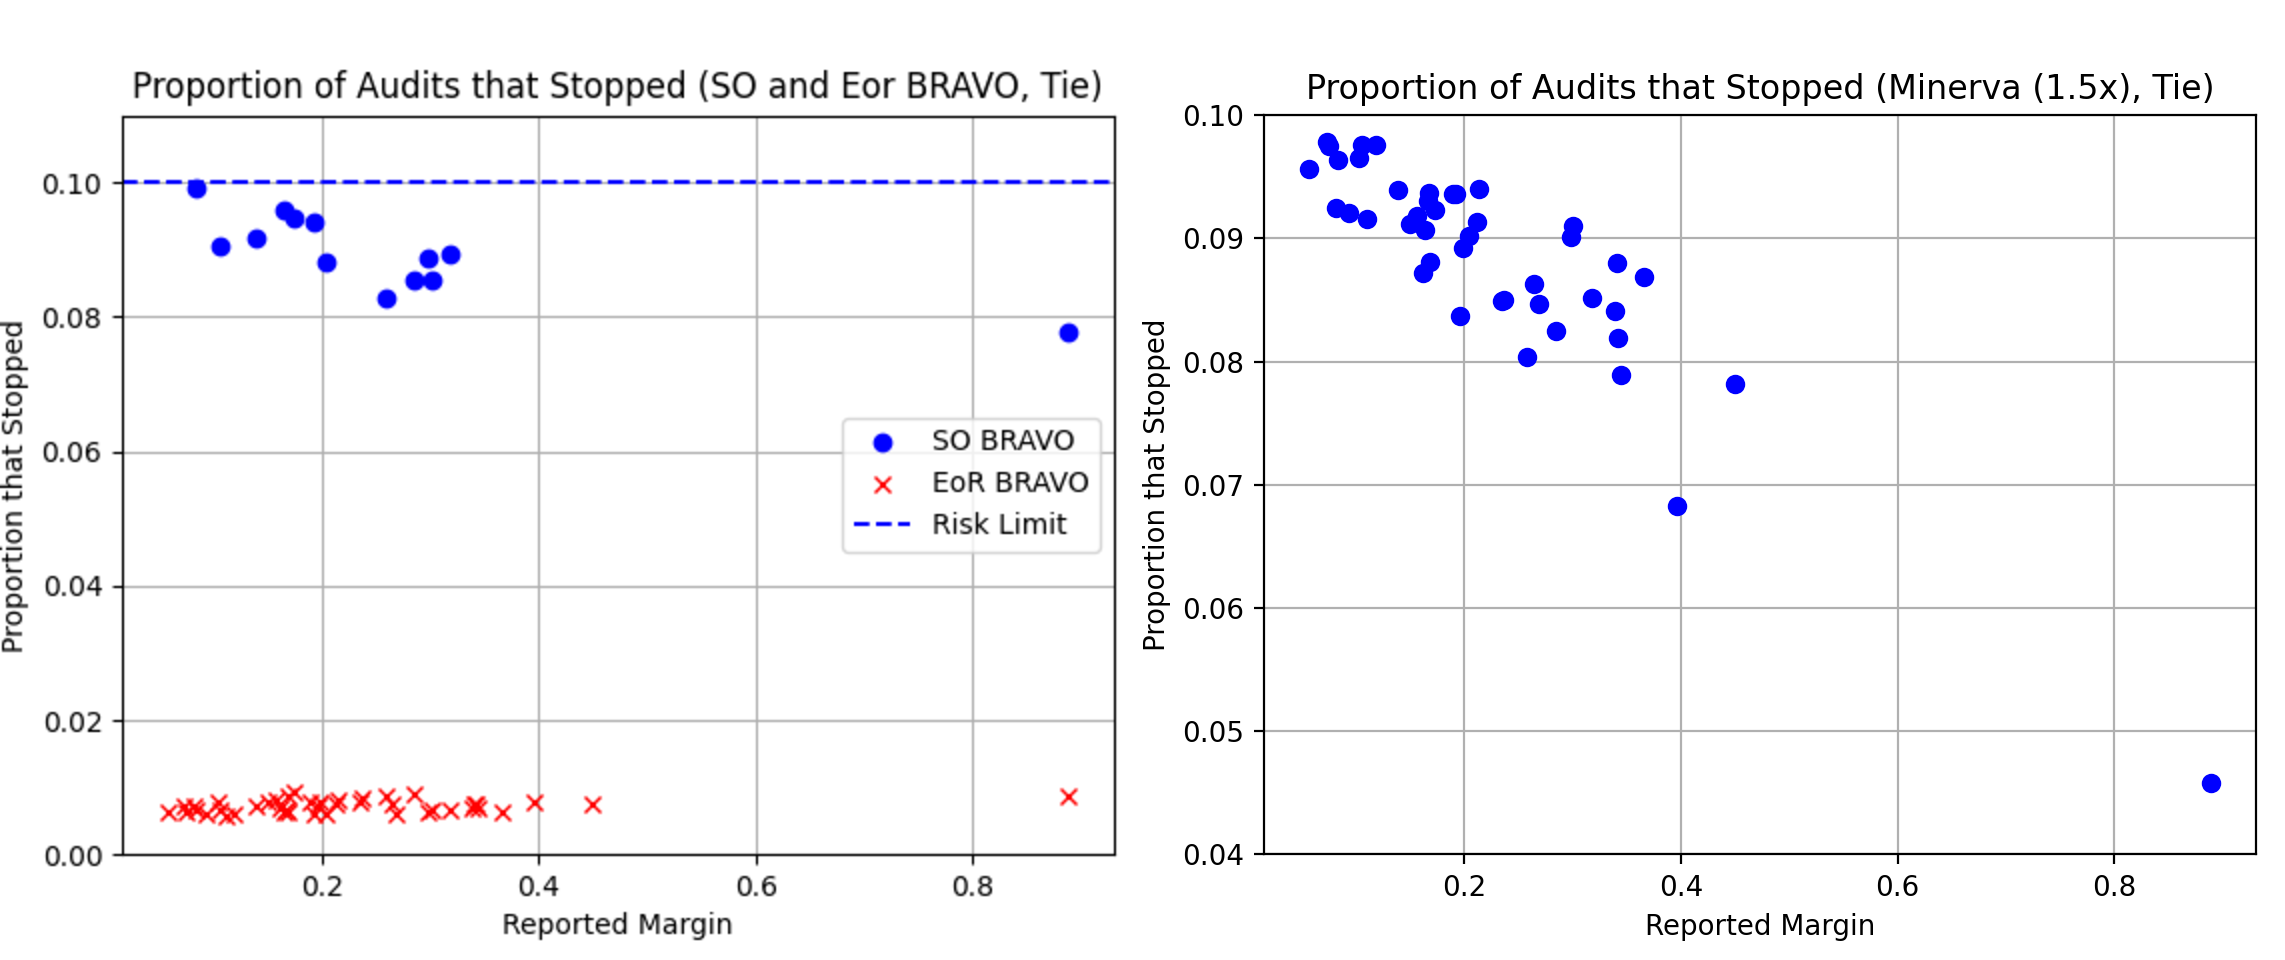
\includegraphics[width=1.07\textwidth]{both_risk_plots.png}
\end{frame}

\begin{frame}
\frametitle{Results: Number of Ballots}

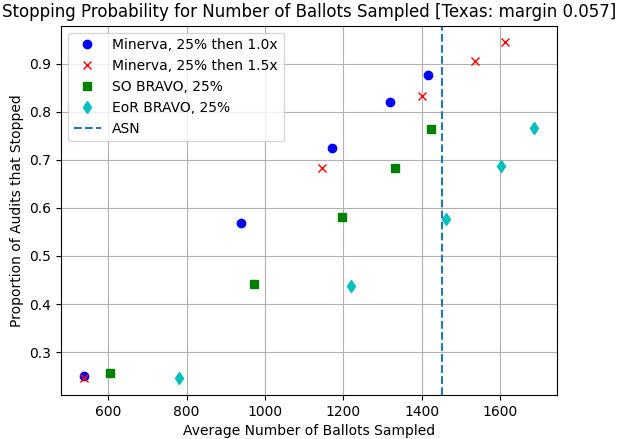
\includegraphics[width=0.5\textwidth]{texas25.png}
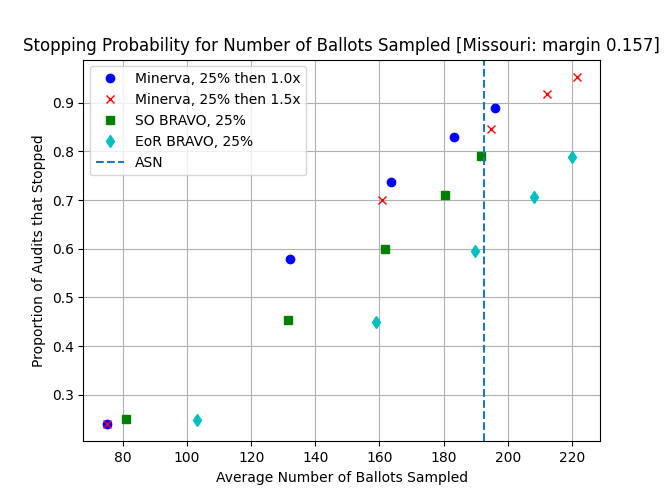
\includegraphics[width=0.5\textwidth]{missouri25.png}

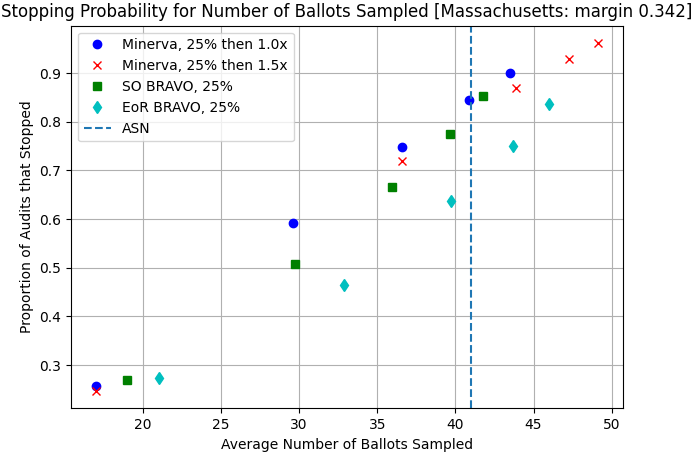
\includegraphics[width=0.5\textwidth]{massachusetts25.png}
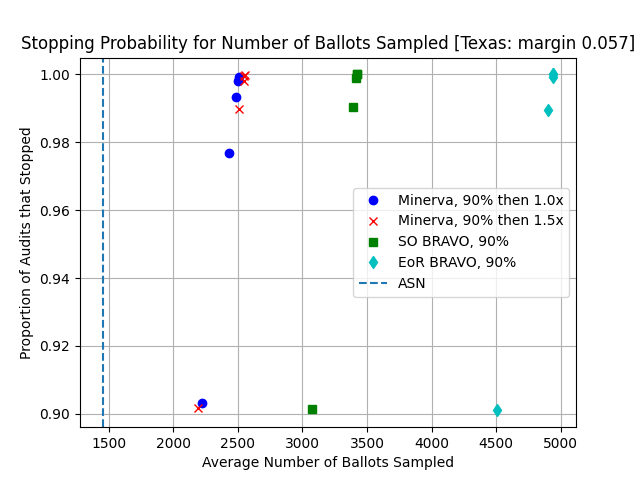
\includegraphics[width=0.5\textwidth]{texas90.png}
\end{frame}

\begin{frame}
\frametitle{Results: Round Size Proportions}

For $\chi_1 = 0.25$, the number of ballots required for \Minerva is smaller than that required by SO \BRAVO and EoR \BRAVO
\begin{itemize}
\item Improvement considerably smaller than that when the stopping probability is $0.9$
\item Number of ballots for SO \BRAVO for $\chi_1 =0.9$ is about a third more than that required by \Minerva, but for $\chi_1 = 0.25$, it requires only about a tenth more ballots than does \Minerva
\item Number of ballots for EoR \BRAVO for $\chi_1 = 0.9$ is about twice those required by \Minerva, but for $\chi_1 =0.25$, it requires only about a fourth to a half more ballots (depending on margin) than does \Minerva

\end{itemize}
For $\chi_1 = 0.9$ with multiplying factor $1$, \Minerva consequent conditional stopping probabilities are about $0.75$ and $0.74$ respectively for rounds two and three. 
\begin{itemize}
\item When the multiplying factor is $1.5$, we see $\chi_2\approx 0.91$
and $\chi_3=0.83$
\end{itemize}

\end{frame}

\begin{frame}
\frametitle{Conclusion}

\begin{itemize}

\item We describe use of the R2B2 library and simulator to characterize: 
\begin{itemize}
\item risk, 
\item stopping probability, and 
\item number of ballots 
\item for various round schedules.
\end{itemize}
\item \Minerva requires fewer ballots than either implementation of \BRAVO in all cases we study, but the advantage decreases for a smaller stopping probability

\end{itemize}

\end{frame}

\begin{frame}
\frametitle{Future Work}
\begin{itemize}
\item More detailed study of the impact of different round schedules
\item Simulations with other underlying distributions
\end{itemize}
\end{frame}


\begin{frame}
\centering 
{Thank you}
\end{frame}



% References?

\end{document}

